\documentclass{standalone}
\usepackage{tikz}
\usetikzlibrary{patterns, positioning}


\begin{document}
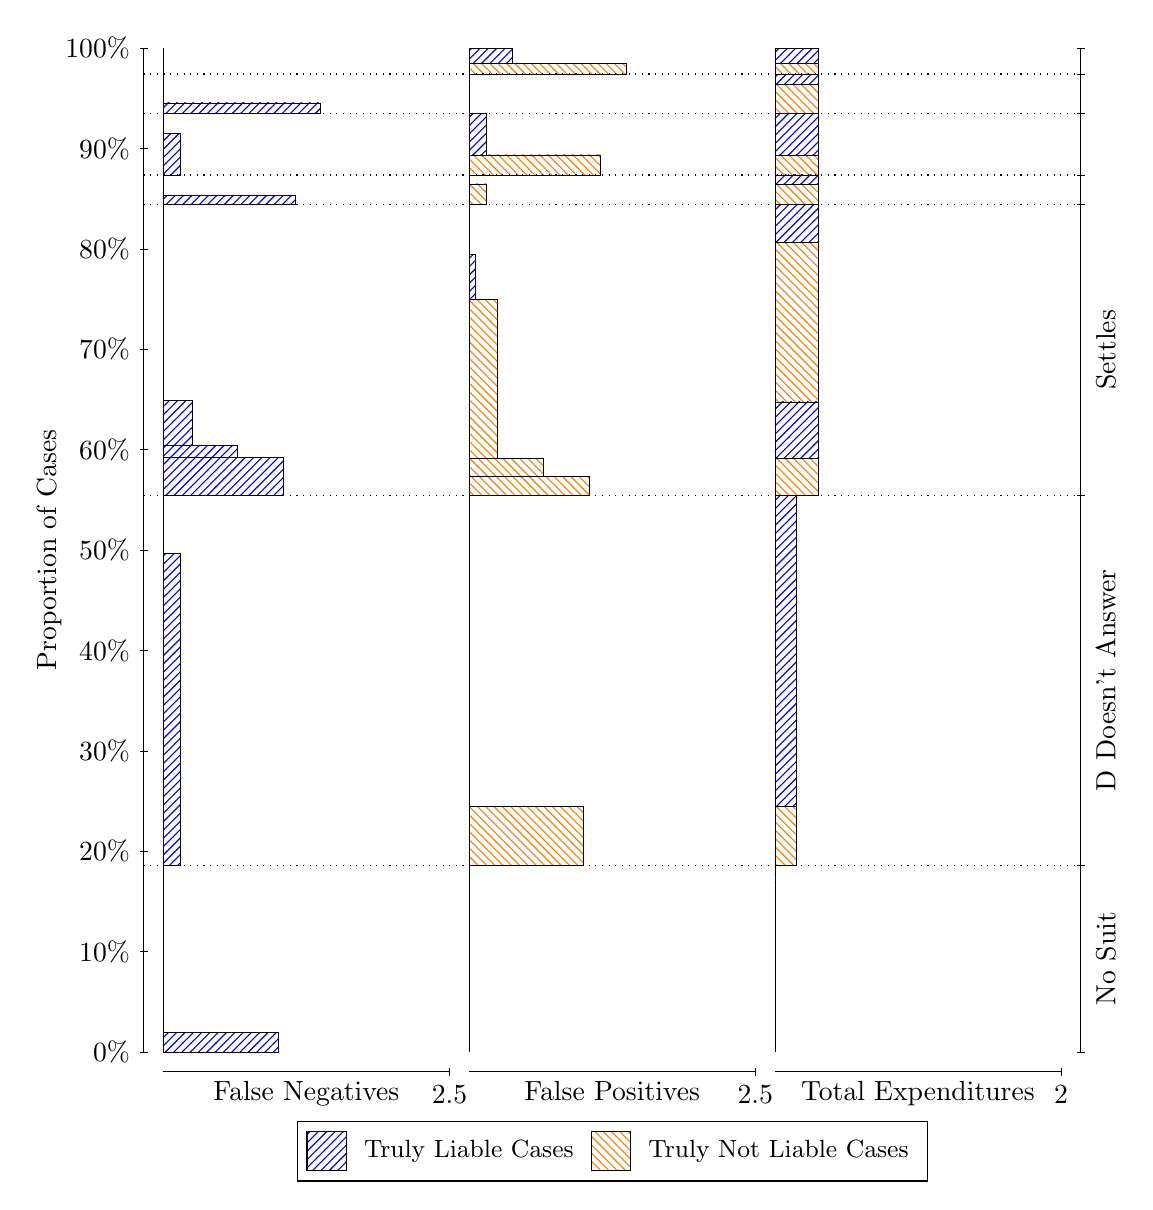
\begin{tikzpicture}
\draw[black, very thin] (1.5,1.75) -- (1.5,14.5);
\node[rotate=90, text=black, anchor=center] at (0.3, 8.125) {Proportion of Cases};
\draw[black, very thin] (1.45,1.75) -- (1.55,1.75);
\node[text=black, anchor=east] at (1.45, 1.75) {0\%};
\draw[black, very thin] (1.45,3.025) -- (1.55,3.025);
\node[text=black, anchor=east] at (1.45, 3.025) {10\%};
\draw[black, very thin] (1.45,4.3) -- (1.55,4.3);
\node[text=black, anchor=east] at (1.45, 4.3) {20\%};
\draw[black, very thin] (1.45,5.575) -- (1.55,5.575);
\node[text=black, anchor=east] at (1.45, 5.575) {30\%};
\draw[black, very thin] (1.45,6.85) -- (1.55,6.85);
\node[text=black, anchor=east] at (1.45, 6.85) {40\%};
\draw[black, very thin] (1.45,8.125) -- (1.55,8.125);
\node[text=black, anchor=east] at (1.45, 8.125) {50\%};
\draw[black, very thin] (1.45,9.4) -- (1.55,9.4);
\node[text=black, anchor=east] at (1.45, 9.4) {60\%};
\draw[black, very thin] (1.45,10.675) -- (1.55,10.675);
\node[text=black, anchor=east] at (1.45, 10.675) {70\%};
\draw[black, very thin] (1.45,11.95) -- (1.55,11.95);
\node[text=black, anchor=east] at (1.45, 11.95) {80\%};
\draw[black, very thin] (1.45,13.225) -- (1.55,13.225);
\node[text=black, anchor=east] at (1.45, 13.225) {90\%};
\draw[black, very thin] (1.45,14.5) -- (1.55,14.5);
\node[text=black, anchor=east] at (1.45, 14.5) {100\%};

\draw[black, very thin] (13.4,1.75) -- (13.4,14.5);
\draw[black, very thin] (13.35,1.75) -- (13.45,1.75);
\node[anchor=west] at (13.35, 1.75) {};
\draw[black, very thin] (13.35,4.1224) -- (13.45,4.1224);
\node[anchor=west] at (13.35, 4.1224) {};
\draw[black, very thin] (13.35,8.822) -- (13.45,8.822);
\node[anchor=west] at (13.35, 8.822) {};
\draw[black, very thin] (13.35,12.51) -- (13.45,12.51);
\node[anchor=west] at (13.35, 12.51) {};
\draw[black, very thin] (13.35,12.888) -- (13.45,12.888);
\node[anchor=west] at (13.35, 12.888) {};
\draw[black, very thin] (13.35,13.668) -- (13.45,13.668);
\node[anchor=west] at (13.35, 13.668) {};
\draw[black, very thin] (13.35,14.17) -- (13.45,14.17);
\node[anchor=west] at (13.35, 14.17) {};
\draw[black, very thin] (13.35,14.5) -- (13.45,14.5);
\node[anchor=west] at (13.35, 14.5) {};

\draw[black, very thin, pattern color=blue, pattern=north east lines] (1.75,1.75) rectangle (3.2033,1.9996);
\draw[black, very thin, pattern color=orange, pattern=north west lines] (1.75,1.9996) rectangle (1.75,4.1224);
\draw[black, very thin, pattern color=blue, pattern=north east lines] (1.75,4.1224) rectangle (1.968,8.0783);
\draw[black, very thin, pattern color=orange, pattern=north west lines] (1.75,8.0783) rectangle (1.75,8.822);
\draw[black, very thin, pattern color=blue, pattern=north east lines] (1.75,8.822) rectangle (3.276,9.3048);
\draw[black, very thin, pattern color=blue, pattern=north east lines] (1.75,9.3048) rectangle (2.6947,9.4494);
\draw[black, very thin, pattern color=blue, pattern=north east lines] (1.75,9.4494) rectangle (2.1133,10.021);
\draw[black, very thin, pattern color=orange, pattern=north west lines] (1.75,10.021) rectangle (1.75,12.51);
\draw[black, very thin, pattern color=blue, pattern=north east lines] (1.75,12.51) rectangle (3.4213,12.624);
\draw[black, very thin, pattern color=orange, pattern=north west lines] (1.75,12.624) rectangle (1.75,12.888);
\draw[black, very thin, pattern color=blue, pattern=north east lines] (1.75,12.888) rectangle (1.968,13.413);
\draw[black, very thin, pattern color=orange, pattern=north west lines] (1.75,13.413) rectangle (1.75,13.668);
\draw[black, very thin, pattern color=blue, pattern=north east lines] (1.75,13.668) rectangle (3.7483,13.804);
\draw[black, very thin, pattern color=orange, pattern=north west lines] (1.75,13.804) rectangle (1.75,14.17);
\draw[black, very thin, pattern color=orange, pattern=north west lines] (1.75,14.17) rectangle (1.75,14.305);
\draw[black, very thin, pattern color=blue, pattern=north east lines] (1.75,14.305) rectangle (1.75,14.5);
\draw[black, very thin, pattern color=orange, pattern=north west lines] (5.6333,1.75) rectangle (5.6333,3.8728);
\draw[black, very thin, pattern color=blue, pattern=north east lines] (5.6333,3.8728) rectangle (5.6333,4.1224);
\draw[black, very thin, pattern color=orange, pattern=north west lines] (5.6333,4.1224) rectangle (7.0867,4.8661);
\draw[black, very thin, pattern color=blue, pattern=north east lines] (5.6333,4.8661) rectangle (5.6333,8.822);
\draw[black, very thin, pattern color=orange, pattern=north west lines] (5.6333,8.822) rectangle (7.1593,9.0598);
\draw[black, very thin, pattern color=orange, pattern=north west lines] (5.6333,9.0598) rectangle (6.578,9.2887);
\draw[black, very thin, pattern color=orange, pattern=north west lines] (5.6333,9.2887) rectangle (5.9967,11.31);
\draw[black, very thin, pattern color=blue, pattern=north east lines] (5.6333,11.31) rectangle (5.706,11.882);
\draw[black, very thin, pattern color=blue, pattern=north east lines] (5.6333,11.882) rectangle (5.6333,12.51);
\draw[black, very thin, pattern color=orange, pattern=north west lines] (5.6333,12.51) rectangle (5.8513,12.774);
\draw[black, very thin, pattern color=blue, pattern=north east lines] (5.6333,12.774) rectangle (5.6333,12.888);
\draw[black, very thin, pattern color=orange, pattern=north west lines] (5.6333,12.888) rectangle (7.3047,13.143);
\draw[black, very thin, pattern color=blue, pattern=north east lines] (5.6333,13.143) rectangle (5.8513,13.668);
\draw[black, very thin, pattern color=orange, pattern=north west lines] (5.6333,13.668) rectangle (5.6333,14.034);
\draw[black, very thin, pattern color=blue, pattern=north east lines] (5.6333,14.034) rectangle (5.6333,14.17);
\draw[black, very thin, pattern color=orange, pattern=north west lines] (5.6333,14.17) rectangle (7.6317,14.305);
\draw[black, very thin, pattern color=blue, pattern=north east lines] (5.6333,14.305) rectangle (6.1783,14.5);
\draw[black, very thin, pattern color=orange, pattern=north west lines] (9.5167,1.75) rectangle (9.5167,3.8728);
\draw[black, very thin, pattern color=blue, pattern=north east lines] (9.5167,3.8728) rectangle (9.5167,4.1224);
\draw[black, very thin, pattern color=orange, pattern=north west lines] (9.5167,4.1224) rectangle (9.7892,4.8661);
\draw[black, very thin, pattern color=blue, pattern=north east lines] (9.5167,4.8661) rectangle (9.7892,8.822);
\draw[black, very thin, pattern color=orange, pattern=north west lines] (9.5167,8.822) rectangle (10.062,9.2887);
\draw[black, very thin, pattern color=blue, pattern=north east lines] (9.5167,9.2887) rectangle (10.062,10.005);
\draw[black, very thin, pattern color=orange, pattern=north west lines] (9.5167,10.005) rectangle (10.062,12.027);
\draw[black, very thin, pattern color=blue, pattern=north east lines] (9.5167,12.027) rectangle (10.062,12.51);
\draw[black, very thin, pattern color=orange, pattern=north west lines] (9.5167,12.51) rectangle (10.062,12.774);
\draw[black, very thin, pattern color=blue, pattern=north east lines] (9.5167,12.774) rectangle (10.062,12.888);
\draw[black, very thin, pattern color=orange, pattern=north west lines] (9.5167,12.888) rectangle (10.062,13.143);
\draw[black, very thin, pattern color=blue, pattern=north east lines] (9.5167,13.143) rectangle (10.062,13.668);
\draw[black, very thin, pattern color=orange, pattern=north west lines] (9.5167,13.668) rectangle (10.062,14.034);
\draw[black, very thin, pattern color=blue, pattern=north east lines] (9.5167,14.034) rectangle (10.062,14.17);
\draw[black, very thin, pattern color=orange, pattern=north west lines] (9.5167,14.17) rectangle (10.062,14.305);
\draw[black, very thin, pattern color=blue, pattern=north east lines] (9.5167,14.305) rectangle (10.062,14.5);
\draw[black, dotted] (1.5,4.1224) -- (13.4,4.1224);
\draw[black, dotted] (1.5,8.822) -- (13.4,8.822);
\draw[black, dotted] (1.5,12.51) -- (13.4,12.51);
\draw[black, dotted] (1.5,12.888) -- (13.4,12.888);
\draw[black, dotted] (1.5,13.668) -- (13.4,13.668);
\draw[black, dotted] (1.5,14.17) -- (13.4,14.17);
\draw[black, very thin] (1.75,1.5) -- (5.3833,1.5);
\node[text=black, anchor=north] at (3.5667, 1.5) {False Negatives};
\draw[black, very thin] (5.3833,1.45) -- (5.3833,1.55);
\node[text=black, anchor=north] at (5.3833, 1.45) {2.5};

\draw[black, very thin] (5.6333,1.5) -- (9.2667,1.5);
\node[text=black, anchor=north] at (7.45, 1.5) {False Positives};
\draw[black, very thin] (9.2667,1.45) -- (9.2667,1.55);
\node[text=black, anchor=north] at (9.2667, 1.45) {2.5};

\draw[black, very thin] (9.5167,1.5) -- (13.15,1.5);
\node[text=black, anchor=north] at (11.333, 1.5) {Total Expenditures};
\draw[black, very thin] (13.15,1.45) -- (13.15,1.55);
\node[text=black, anchor=north] at (13.15, 1.45) {2};

\node[text=black, centered, rotate=90] at (13.72, 2.9362) {No Suit};
\node[text=black, centered, rotate=90] at (13.72, 6.4722) {D Doesn't Answer};
\node[text=black, centered, rotate=90] at (13.72, 10.666) {Settles};





\draw (7.449999999999999,1.5) node[draw=none] (baseCoordinate) {};
\begin{scope}[align=center]
        \matrix[scale=0.5, draw=black, below=0.5cm of baseCoordinate, nodes={draw}, column sep=0.1cm]{
            \node[rectangle, draw, minimum width=0.5cm, minimum height=0.5cm, pattern color=blue, pattern=north east lines] {}; &
            \node[draw=none, font=\small, text=black] (B) {Truly Liable Cases}; &
            \node[rectangle, draw, minimum width=0.5cm, minimum height=0.5cm, pattern color=orange, pattern=north west lines] {}; &
            \node[draw=none, font=\small, text=black] (B) {Truly Not Liable Cases}; \\
            };
\end{scope}

\end{tikzpicture}
\end{document}